\documentclass[12pt]{article}
\usepackage{listings}
\usepackage[colorlinks=true,pagebackref,linkcolor=blue]{hyperref}
\usepackage{graphicx}
\textwidth=7in
\textheight=9.5in
\topmargin=-1in
\headheight=0in
\headsep=.5in
\hoffset  -.85in

\lstset{
basicstyle=\footnotesize\ttfamily,
language=bash,
upquote=true,
breakatwhitespace=true,
columns=fullflexible,
keepspaces,
%numbers=none,
tabsize=3,
frame=blrt,
framextopmargin=5pt,
showstringspaces=false,
extendedchars=true
}

\pagestyle{empty}

\renewcommand{\thefootnote}{\fnsymbol{footnote}}

\begin{document}



\begin{center}
{\bf AMS 550.400 \quad HW SET 1\quad  Due Date:  Oct 8}\\
\vskip.2in
{\footnotesize Last Compiled on \today}
\end{center}

\setlength{\unitlength}{1in}

\begin{picture}(6,.1) 
\put(0,0) {\line(1,0){6.25}}         
\end{picture}

 

\renewcommand{\arraystretch}{2}

\noindent\textbf{General Instruction:} 
To complete the homework set, you are required to do the followings. 
Your solutions must be typed in \LaTeX\ using the course homework
template.  
The progression of your homework solution is to be
``recorded'' by making a git folder specifically for this homework
set.  The burden of proof is on you, and if your git commit history
is sparse, then you may be liable for a penalty.  
A paper copy of the PDF output of your \LaTeX\ file is 
to be submitted to your instructor in class on the due date.
\emph{After} submitting the paper copy, but \emph{before} the end of
the due date, you will upload your work to your github by making a remote repository
specifically for the homework, and post the link to the repository 
at the designated \emph{Discussion} forum in Blackboard by making 
a thread just for you.  The repository name in your github should be
\texttt{550400.homeworkset.1} and the discussion forum thread should
be named \texttt{YourFirstNameMiddleInitialLastName}, e.g.,
\texttt{BaracHObama} and \texttt{WillardMRommey}. 
You have till the end of 
the due date to finalize your github repository.  
However, any commit made after the class time of the due date will be 
inadmissible. \emph{Your attention to details in following this instruction will be 
critical, and if not followed exactly at the time of collection, the
homework set may be graded at $90\%$ of the full score}.

\vskip.25in
\noindent\textbf{Problem 1 (10 pts):}  
Assume that you are starting from ``scratch'' at the directory \verb+~/+.
Provide a sequence of git/bash commands that yields a git folder with 
a commit history such that:
\begin{itemize}
\item the \emph{master} branch has commits $A$, $B$, $C$, $X$ and $D$,
\item the \emph{alt} branch has commits $A$, $B$, $X$,
\end{itemize}
Suppose that you are currently working on \texttt{master} branch. Draw 
its commit history graph (i.e., the graph portion of the output of
\verb+git log --graph --oneline+).  Next, assume that 
you are on \texttt{alt} branch. Draw its commit history graph.  

\bigskip
\noindent\textbf{Answer to Problem 1:}\\
Commands:\\
\verb+mkdir problem1.git+\\
\verb+cd problem1.git+\\
\verb+git init .+\\
\verb+vi main.txt+ (Input A in the text)\\
\verb+git add .+\\
\verb+git commit -m "A is done"+\\
\verb+vi main.txt+ (Input B in the text.)\\
\verb+git add .+\\
\verb+git commit -m "B is done"+\\
\verb+git branch alt+\\
\verb+git checkout alt+\\
\verb+vi main.txt+ (Input X in the text.)\\
\verb+git add .+\\
\verb+git commit -m "X is done"+\\
\verb+git checkout master+\\
\verb+vi main.txt+ (Input C in the text.)\\
\verb+git add .+\\
\verb+git commit -m "C is done"+\\
\verb+git merge alt+\\
\verb+git commit -a+\\
\verb+vi main.txt+ (Clean the content and input D in the text.)\\
\verb+git add .+\\
\verb+git commit -m "D is done"+\\


\noindent{To see its commit history graph on master branch, type in the following command:}\\
\verb+git log --graph --oneline+\\
and the graph is in Figure 1.

\begin{figure}[htb]
    \begin{center}
        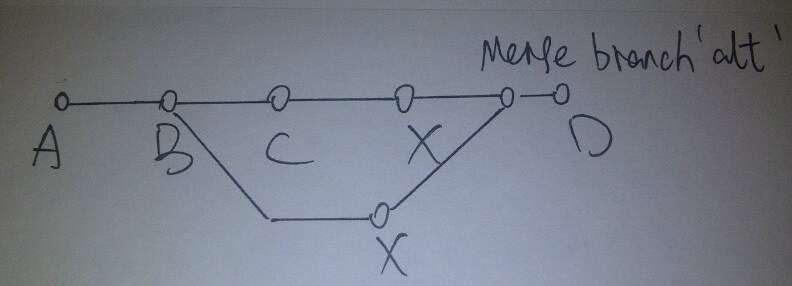
\includegraphics[width=0.75\textwidth]{figure1.png}
    \end{center}
    \caption{on Master Branch--Commit History Graph}
\end{figure}

\noindent{Checkout to alt branch, type in the following commands and see its commit graph history:}\\
\verb+git checkout alt+\\
\verb+git log --graph --oneline+\\
and the graph is in Figure 2.

\begin{figure}[htb]
    \begin{center}
        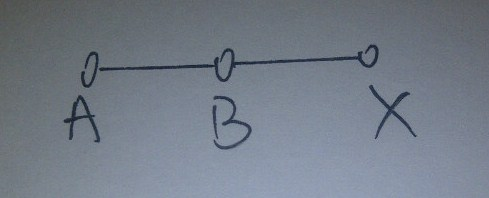
\includegraphics[width=0.5\textwidth]{figure2.png}
    \end{center}
    \caption{on Alt Branch--Commit History Graph}
\end{figure}

\vskip.25in
\noindent\textbf{Problem 2 (10 pts):}
Assume that you are starting from ``scratch'' at the directory \verb+~/+.
Provide a sequence of git/bash commands that yields a git folder and 
\begin{itemize}
\item configure your git with your name and your email address,
\item set up an alias for each of the git remotes listed below:
\begin{verbatim}
git://github.com/nhlee/550400.stanza1.git 
git://github.com/nhlee/550400.stanza2.git 
git://github.com/nhlee/550400.stanza3.git 
\end{verbatim}
Assume that each remote contains exactly single commit with 
a txt file for a single (different) stanza,
\item pull to combine three stanzas of a poem,
\item after the first pull, add the title of the poem,
\item after the second and third pull, resolve the merge conflict,
\item after resolving the third pull merge conflict, push the result
  to your (newly created) remote repository. 
\end{itemize}

\bigskip
\noindent\textbf{Answer to Problem 2:}\\
To configure my git with my name and email address, type in the following commands:\\
\verb+git config --global user.email ydu10@jhu.edu+\\
\verb+git config --global user.name "Yu Du"+\\

\noindent{}\\
\verb+mkdir problem2.git+\\
\verb+cd problem2.git+\\
\verb+git init .+\\
\verb+vi main.txt+ (Input something at the begining)\\
\verb+git add .+\\
\verb+git commit -m "Start"+\\
\verb+git remote add ford git://github.com/nhlee/550400.stanza1.git+\\
\verb+git pull ford master+\\
\verb+vi main.txt+ (Clean the text and add a title.)\\
\verb+git add .+\\
\verb+git commit -m "1 is done"+\\
\verb+git remote add toyota git://github.com/nhlee/550400.stanza2.git+\\
\verb+git pull toyota master+\\
\verb+git commit -a+\\
\verb+vi main.txt+ (Clean the text.)\\
\verb+git add .+\\
\verb+git commit -m "2 is done"+\\
\verb+git remote add saab git://github.com/nhlee/550400.stanza3.git+\\
\verb+git pull saab master+\\
\verb+git commit -a+\\
\verb+vi main.txt+ (Clean the text.)\\
\verb+git add .+\\
\verb+git commit -m "3 is done"+\\
\verb+git remote add work git://github.com/yangxiaohan/550400.homeworkset.1.git+\\
\verb+git push work master+\\

\newpage
\noindent\textbf{Problem 3 (40 pts):}
Consider a team of four students, say, $A$, $B$, $C$ and $D$, 
who just started working 
on writing a \texttt{latex/beamer} file, say \texttt{main.tex}, 
for a class presentation of their work statement.  
Assume that they do not wish to coordinate their schedules for a
concurrent group meeting (both virtually and physically).  
Assume that:
\begin{itemize}
\item $A$ is in charge of \emph{Introduction},
\item $B$ is of \emph{Problem Statement}, 
\item $C$ is of  \emph{Timeline},
\item $D$ is of \emph{Deliverable} part of the presentation.  
\end{itemize}
In other words, their contributions to \texttt{main.tex} do not overlap.
Then, 
\begin{itemize}
\item first, devise a work flow strategy for the team so that they can
  collaborate asynchronously using \texttt{git},
\item next, devise yet another \texttt{git} strategy different from your earlier
  proposal.  
\end{itemize}
Finally,
\begin{itemize}
\item discuss the strength and weakness of each of your proposed strategies in terms of merge
conflicts resolution,
\item make the final recommendation.  
\end{itemize}
In order to answer this question, \emph{build}
a mathematical model, \emph{following} the guideline from IMM. 
Use Section 1.4 and Section 1.5 of IMM as \emph{role models}.    
For example, you are to identify which variables  are exogenous 
and which are endogenous.  More specifically, among other things, 
in your model, is the preamble part of \texttt{main.tex} an endogenous 
or exogenous variable?  
Note also that in addition to this issue, there are other issues that
you are to consider.  So, \emph{be sure to consult IMM}. 

\newpage
\noindent\textbf{Answer to Problem 3:}\\
\\
\noindent\textbf{Strategy One:}\\
Strategy One is to initiate a git folder at master to start this project. At the second node, there are four branches corresponding to four different students. A branch is working on \emph{Introduction}, B branch is working on \emph{Problem Statement}, C branch is working on \emph{Timeline} and D branch is working on \emph{Deliverable}. And at the end when each of them finishes his/her part, they need to pull from the master first, merge and then push to the master in order not to leave out the other people's work. This Strategy is illustrated in Figure 3.

\begin{figure}[htb]
    \begin{center}
        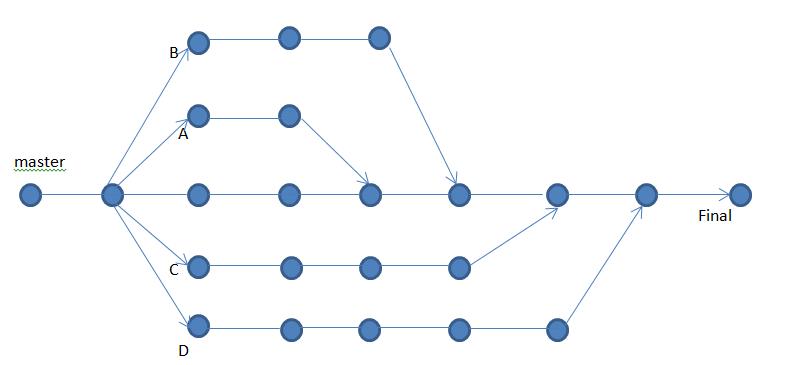
\includegraphics[width=0.75\textwidth]{figure3.png}
    \end{center}
    \caption{Strategy One}
\end{figure}

\noindent\textbf{Strategy Two:}\\
For strategy two, each of them is doing the work on their own until they finish their parts. And then a random person A or B or C or D can set up an initial git folder on master and then pull and merge for each of them. Start with A \emph{Introduction}, pull, add and commit.Then pull B's work \emph{Problem Statement}, solve the merging conflicts manually and add and commit.The next is to pull C's work \emph{Timeline}, solve the merging conflicts manually and add and commit.The last is to pull D's work \emph{Deliverable}, solve the merging conflicts manually and add and commit. \\
 This Strategy is illustrated in Figure 4.


\begin{figure}[htb]
    \begin{center}
        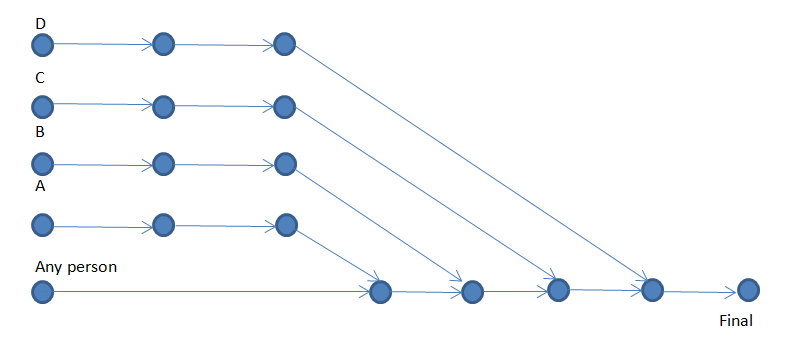
\includegraphics[width=0.75\textwidth]{figure4.png}
    \end{center}
    \caption{Strategy Two}
\end{figure}
We are interested in knowing which strategy is better in terms of doing a good job on time efficiency as well as merging issues. Git is a creative tool that provides people with the opportunity to work asynchronously while at the end to deliver the complete final product. So when we come to the final product, it means that we need to merge each person's work together, which might raise some of the merging issues. In addition, there are multiple ways and strategies to achieve a final product.Therefore our goal is to find a strategy that could solve these merging conflicts more efficiently.

The above are two strategies that both could deliver a complete final product. And we know that the only things we are concerned about are the merging of four parts: Introduction, Problem Statement, Timeline as well as deliverable. We do not focus on the other parts of main.txt which might be a short beginning or a conclusion. So those are considered exogenous variables in this context. Therefore we ignore the other parts of main.txt than the four core parts.

For Strategy One, each person is working on their own branch and no one is influenced by the other one. When they are ready to submit their parts, they first need to pull from the master and do a merging with other person's work. Then make a push to the master to include his/her work.In this way nobody's work will be left behind and each person is responsible for doing a pull, merge and push to have a complete final product.

For Strategy Two, each person is doing his/her part on their own computer. At the time they are finished, a random person A or B or C or D come to pull each one's work and merge manually to be a complete final product.

For me, the Strategy One is better because each of the person can do a pull, merge and push. There is indeed no need for a random person to be specifically responsible for all the pull and merge. To test the model we can simply assign some words or sentences for each of the four parts and then do a merge according to the above two strategies to assess which one is better in terms of merging issues.





\newpage
\vskip0.25in
\noindent\textbf{Problem 4 (aka.\ Fair Play, 40 pts):}
Answer the following question:
\begin{verse}
Is the tennis game fair?
\end{verse}
Note that unlike Problem 3, this question is vaguely stated.
This is intensional, whence to begin, you will first need to clarify
what exactly your question is.
You may use the class discussion on this particular 
problem, but you \emph{may not} directly refer to our 
discussion.  Instead, formulate the model carefully but concisely in 
your own words.   

\newpage
\noindent\textbf{Answer to Problem 4:}\\

\noindent\textbf{Formulate the Problem}\\
The original problem we are going to investigate is that whether the tennis game is fair. In order to know whether or not the game is fair the first thing we need to do is to know the rules of this tennis game and in what way we assess the fairness. In tennis game, opponents stand on opposite sides of the court. The player who delivers the ball to start the point is called the server. The player who stands opposite and cross-court from the server is the receiver.  The server always calls his score first. If the server wins the first point, he gets a score of 15. Scoring is done like a clock (LOVE--15--30--40--45).Love means zero in tennis. The second point is called 30. The third point is called 40 and game is won when the score goes to 45. If the score is 40-40, also known as deuce, one side must win by two points. Advantage-In means if the server wins the next point, he wins the game. Advantage-Out means the receiver has a chance to win the game on the next point. After the game, the opponents serve. Games equal 1. The first to win 6 games, by two, wins the set. The first to win 2 sets wins the match in best of three game. If the score is 6-6, a tie-breaker is played. This is scored by one's. The first side to score 7 points winning by two wins the set. The tiebreaker continues until one side wins by two. Hence, Game-Set-Match.

So now let us consider the meaning of fairness in this context. If Player A is much stronger than Player B regarding the tennis skills, there is no doubt that with a high probabiloity Player A is going to win the game. However, this factor is influenced by the individual and you can barely say much on the fairness of the game itself. Another factor, psychological influence, should also fall into this category which is not influenced by the rule of the game. What the rule says is that after each game, the previous server will become the receiver and the previous receiver will become the new server. Most people would assume that intuitively the server has an advantage in the tennis game because he can start the ball in whatever way he likes and hit the ball with more power from a standing point thus the game is unfair. Therefore in order to check the fairness of the game, it is equivalent to checking whether the probability to win the game favors the server. If say, the server wins the game with probability $p$, and $p=0.5$, therefore the receiver has the probability $1-p$, $1-p=0.5$ as well. Hence, the probability to win the game for the server and the receiver is the same thus to be a server is not going to have the advantage and the tennis game is fair. Suppose an extreme case where the probability to win the game for the server is equal to 1, $p=1$. In this case the server wins all the games and to be a server gurantees that you will win this game for 100\% sure. So the tennis game is not fair and whether to win or not totally depends on whether you are the server or not. Therefore, depending on the probability to win the game for the server, we can assess the fairness of the game. If the probability is equal to 0.5, the game is fair and both sides have equal chances of winning the game. However if the probability is not equal to 0.5 and favors either party, the favored party has a more likelihood to win the game thus the game is not fair.\\

\noindent\textbf{Outline the Model}\\
Carry out statistical experiments to assess the probability to win the game for the server. In this context, we are not going to consider the factors like tennis skills, psychological influence and so on. We are only interested in knowing whether the server has an advantage thus the game is fair or not. Therefore controlling the other factors, we pick up $N$ games from the past history where two players are equivalent in terms of tennis skills, psychological effect. Therefore we do not focus on the specific player instead we focus on the server and the receiver. Let the probability to win a game for the server be $p$ and the probability to lose a game therefore be $1-p$. The probability does not vary with the games. For each game, assign value $1$ to the server if he wins otherwise assign a value $0$. A possible sequence for the result of these $N$ games is like the following:\\


$$\left( \begin{array}{cccccc} Game1 & Game2 & Game3 & Game 4 & \cdots&Game N \\
0 & 1&0&0&\cdots&1 \end{array} \right)$$
\\
We are interested in estimating the proportion of the games where the server wins, which is also the probability to win a game for the server. The point estimate of the probability is the sample mean for the sequence which is the number of wins divided by the total number of games $N$.\\
$$\hat p=\frac{ the~number~of~wins}{N}$$
\\
And the 95\% confidence interval estimate for the probability to win a game for the server is:
$$\mbox{} \left[ \begin{array}{ccc}
\hat p-1.96\sqrt{\frac{\hat p(1-\hat p)}{N}} ,& \hat p+1.96\sqrt{\frac{\hat p(1-\hat p)}{N}}  \end{array} \right]$$\\

It can be seen that we could increase the sample size $N$ in order to narrow down our interval to an optimum level specified. Therefore, if the the estimate of the probability to win a game for the serve is very close to 0.5 we could conclude that the rule of the game is fair. To be a server does not give the person the advantage in the game. If the estimate is far away from 0.5 we could say that each game favors the server. The server has a higher likelihood of winning the game than the receiver thus the rule of the game is unfair.

In this case, exogenous variables are the skill levels of the players as well as their psychological factors. If Player A is much stronger than Player B regarding the tennis skills, there is no doubt that with a high probabiloity Player A is going to win the game. However, this factor is influenced by the individual and you can barely say much on the fairness of the game itself. Another factor, psychological influence, should also fall into this category which is not influenced by the rule of the game. Since we are interested in investigating the fairness of the game itself, we will check if the server has an advantage to win the game thus whether or not the server has the advantage to win the game becomes our endogenous focus. Causality is the relationship between an event (the cause) and a second event (the effect), where the second event is understood as a consequence of the first. Here the first event can be considered as the player being a server and the second event be whether or not that player wins the game thus to see if there is a causality between being the server and winning the game, if the server has an advantage to win the game.\\


\noindent\textbf{Is it useful?}\\
In the ideal world, it indeed makes sense to assess the probability to win a game for the server while holding other variables constant like tennis skills and psychological effect. But in the real world it is hard to do so. There will never be two players who are at the same level of skills and have the same psychological factors. And the result of the game will be in a large extent influenced by these variables. But actually we could do a computer simulation where we set up everything perfectly to avoid the influence of the above variables and then assess if the server has the advantage following the model.\\

\noindent\textbf{Test the Model}\\
When we derive a conclusion that the server has an advantage or not by following the above model, we can still collect more data regarding two equivalent players and do a new interval estimate to see if there is a significant change big enough to change our conclusion.












\newpage
\vskip0.25in
\noindent\textbf{Final Remarks about Problem 3 \& Problem 4:} 
They are open-ended problems.  However, your scores will be determined
by how well do you follow the exposition style outlined by IMM and
WMA.  For both problems, your write-up should be 
\begin{itemize}
\item self-contained,
\item covering all four parts of Section 1.3 of IMM,
\item paying a particular attention to any causal relation that you
  might be investigating, following Chapter 3 of WMA,
\item answering questions that are explicitly asked in the problem statements.
\end{itemize}
For Problem 3, focus mostly on Step 2 and Step 3 of Section
1.3 of IMM.  For Problem 4, focus mostly on Step 1 and Step
2.  For each problem, minimum 1 pages and maximum 2 pages.
\end{document}
